\chapter{Experimental Evaluations}

In chapters 3 and 4, we have discussed the architecture and the calibration applied to the system.  The main objective of the study was to compare how closely the calibrated data values from the low-cost sensor network are to that of the reference system located at the Plaza 400 building, downtown Prince George. The sensor system was deployed for six days from 30 May, 2019 to 4 June, 2019 and the calibrated data was collected and later compared to the values from the reference system. Before getting into the deployment section, we will briefly describe the complete system and will show how the data values are collected from our sensor system.



The Arduino microcontroller is connected to five sensors and these sensors collects the values for a fixed interval of time, in our case we have collected values for every five minutes and taken the hourly average of that data which gives 24 data points for a day. These sensor readings are digitized by the Arduino and a set of equations are applied to the raw signal and converted to concentration values. In the initial cycle, which is the calibration process, we collect these concentration values and supply them to the MAT tool for calibration. Once the regression equations are determined, we supply these to the Arduino to get subsequent calibrated values. The complete flow diagram of the system is as shown in Figure \ref{flow}. Further, we will be discussing the comparison between the calibrated values from the sensor system to the data collected from the reference station. 
These are the observations that we have obtained after we have put our system out for six days. We have also added the weather data which includes the temperature, humidity and sunlight data in Prince George during the measured days in the Appendix section for reference.




\begin{figure}[h]
  \begin{center}
  %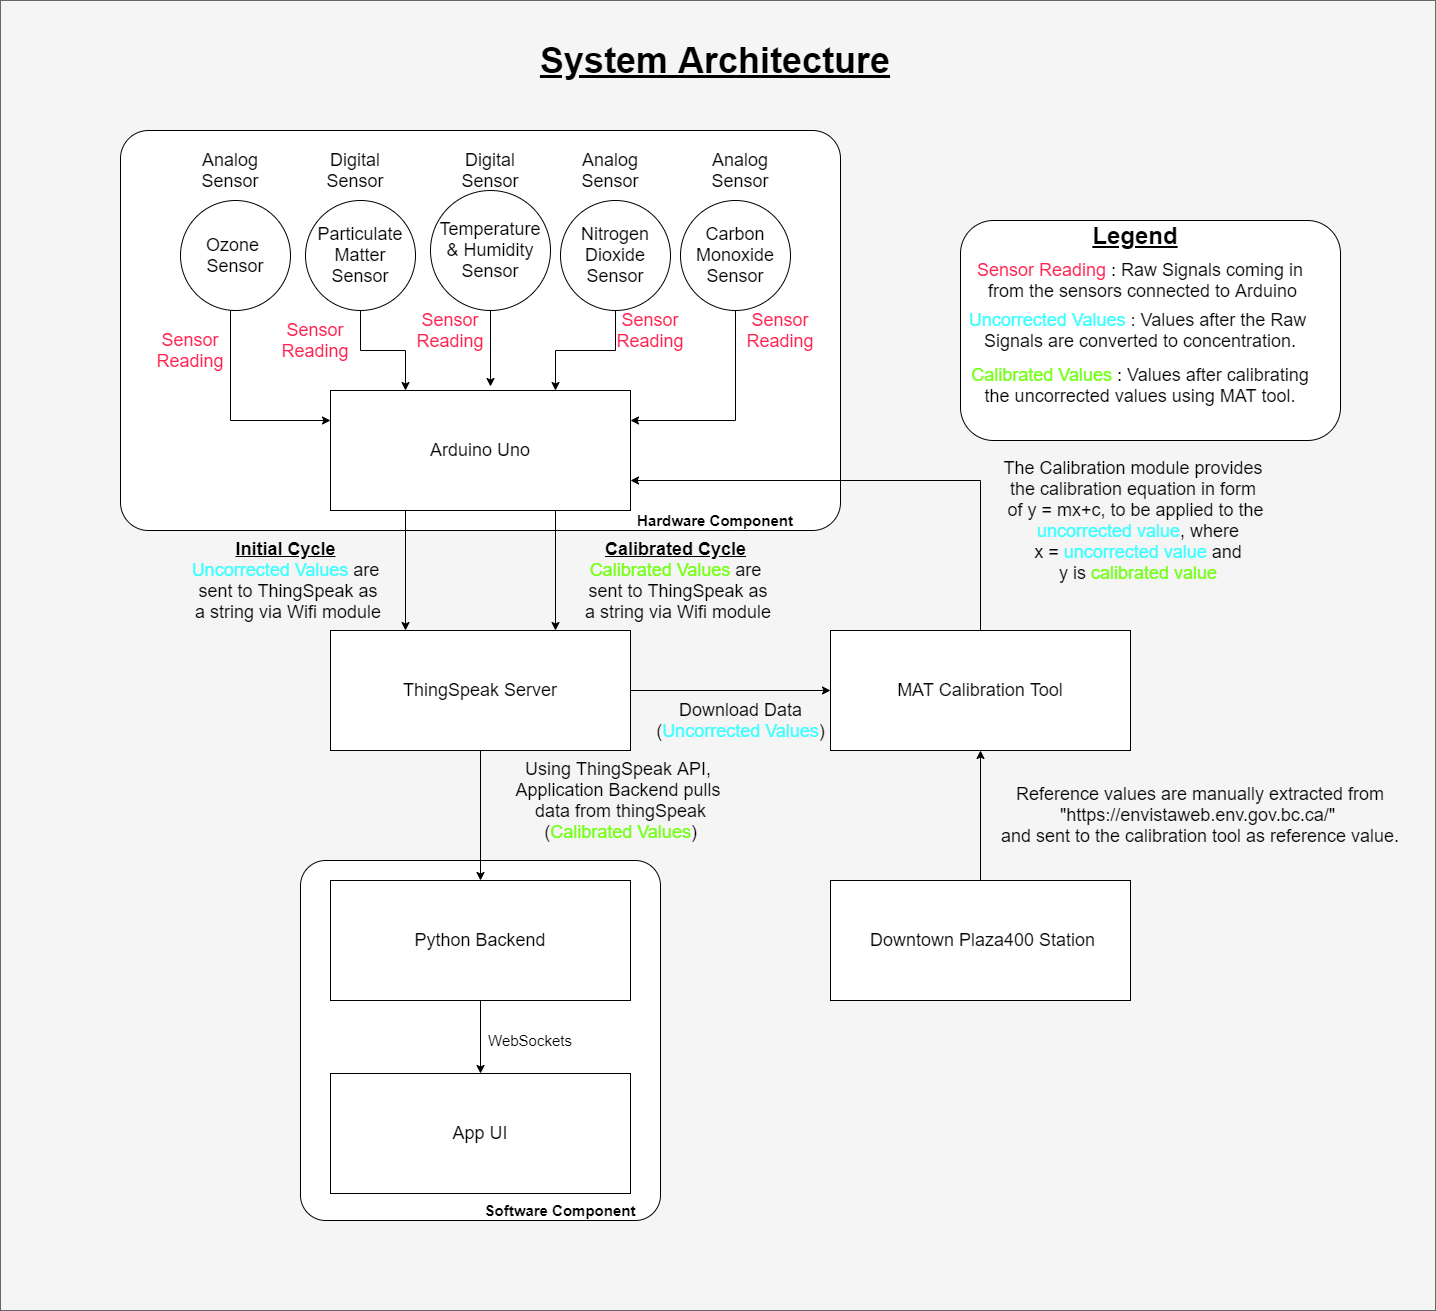
\includegraphics[scale=0.26]{images/figure68.png}
  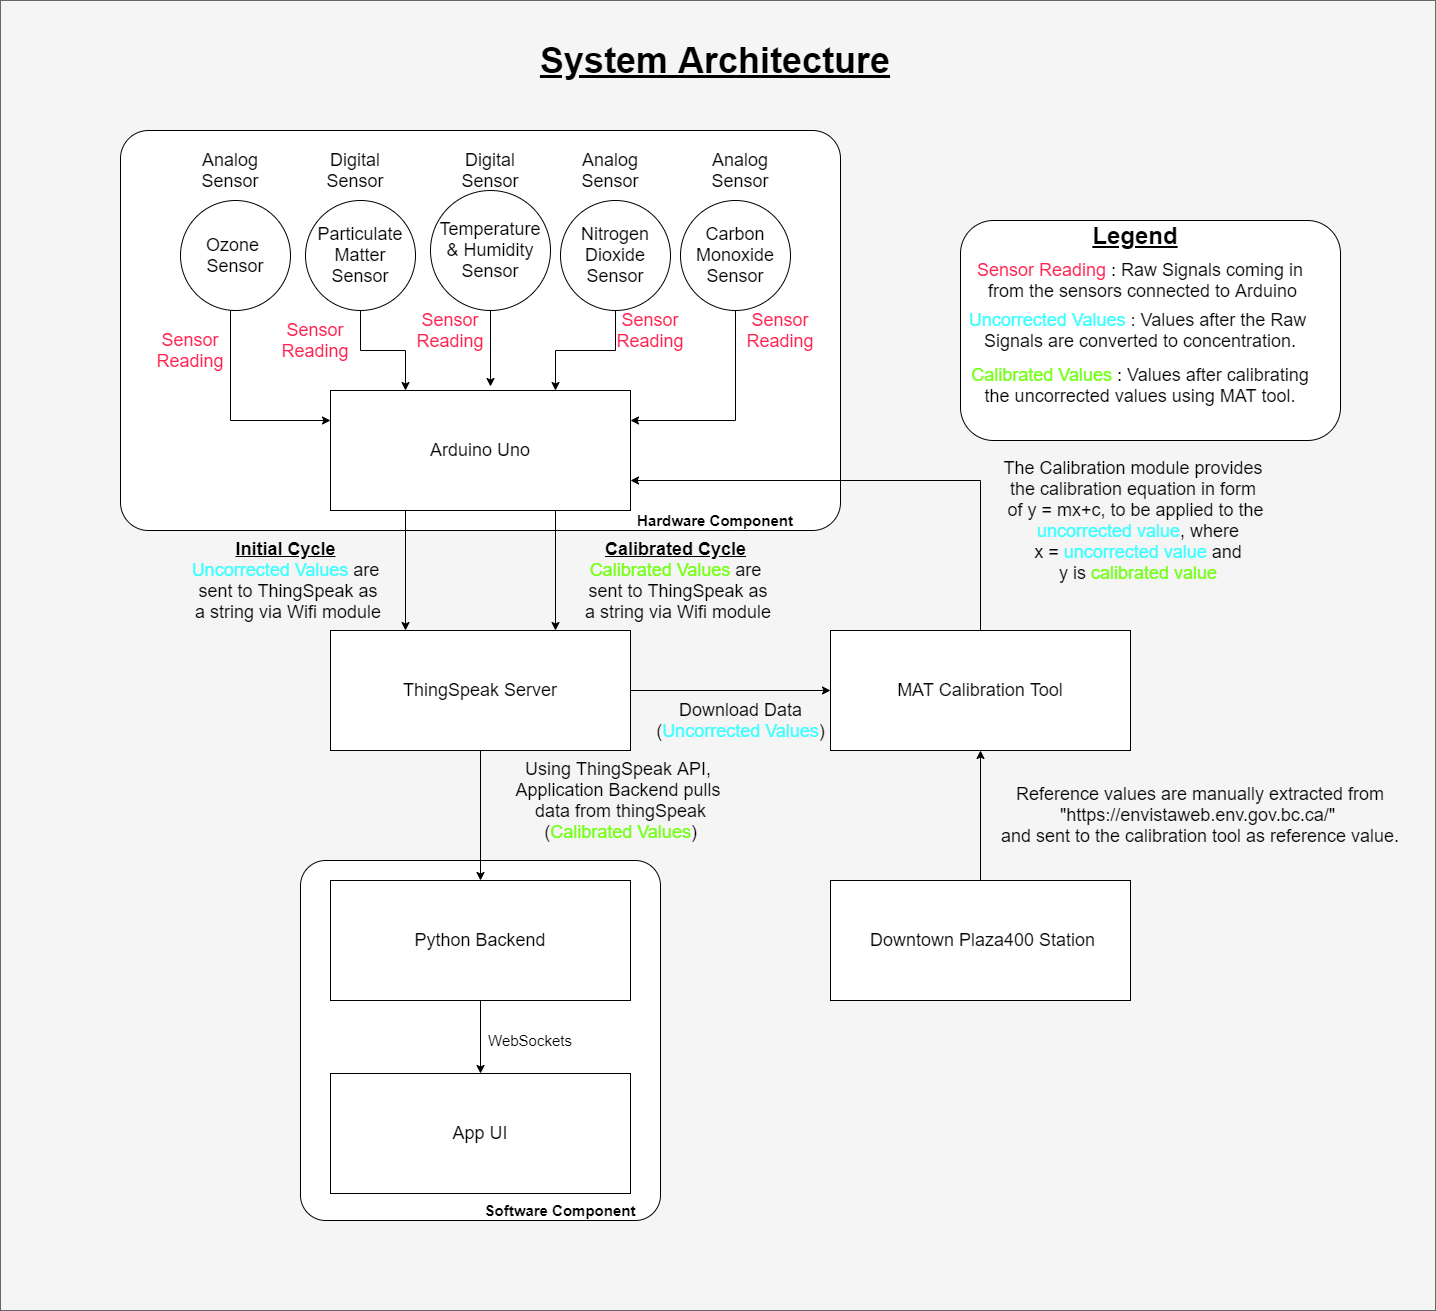
\includegraphics[width=15.50cm,height=18.20cm]{images/figure68.png}
  \end{center}
  \caption{The complete flow diagram showing the hardware and the software of the developed sensor system}
  \label{flow}
  \hspace{1 cm}
\end{figure}


\clearpage

\begin{comment}
The Arduino is connected with five sensors out of these sensors the particulate sensor is a Digital sensor, and the rest are Analog sensors. In the case of Analog sensors, when there is a change in concentration of the gases the sensor resistance changes and hence fluctuates the output voltage. This output voltage can be referred to as raw measurement or raw data. Initially, the system was made to collect these raw measurements by keeping the system out for two days. Once the raw measurements were collected we applied the calibration procedure to these measurements using MAT. By calibrating we are trying to create a linear relationship between the reference system and our low-cost sensor system. The linear equation from MAT is then applied to the subsequent raw data to obtain the calibrated data outputs. 

In the case of a Digital sensor (Particulate matter), the output is \lq{amount of particle}\rq which is converted to \lq{mass of particle }\rq using a generic formula. Here the raw data or raw measurements are not voltage values but the mass of the particle. To this \lq{mass of particle}\rq, the calibration is applied and the calibrated data outputs are obtained.
\end{comment}









\section{Deployment}

To understand the performance of our system, we deployed the air pollution monitoring system for eight days in College Heights, Prince George in which the first two days the raw data from the system was used for calibration and the following six days for measurement. Figure \ref{deployed} shows the experimental set up of the sensor system deployed at the location. The system was directly connected to a power cable and was hung over a platform. The collected values were transferred to the ThingSpeak database through the WiFi module in an hourly averaged form and hence 24 data points were collected for each day.

\begin{figure}[h]
    \begin{center}
    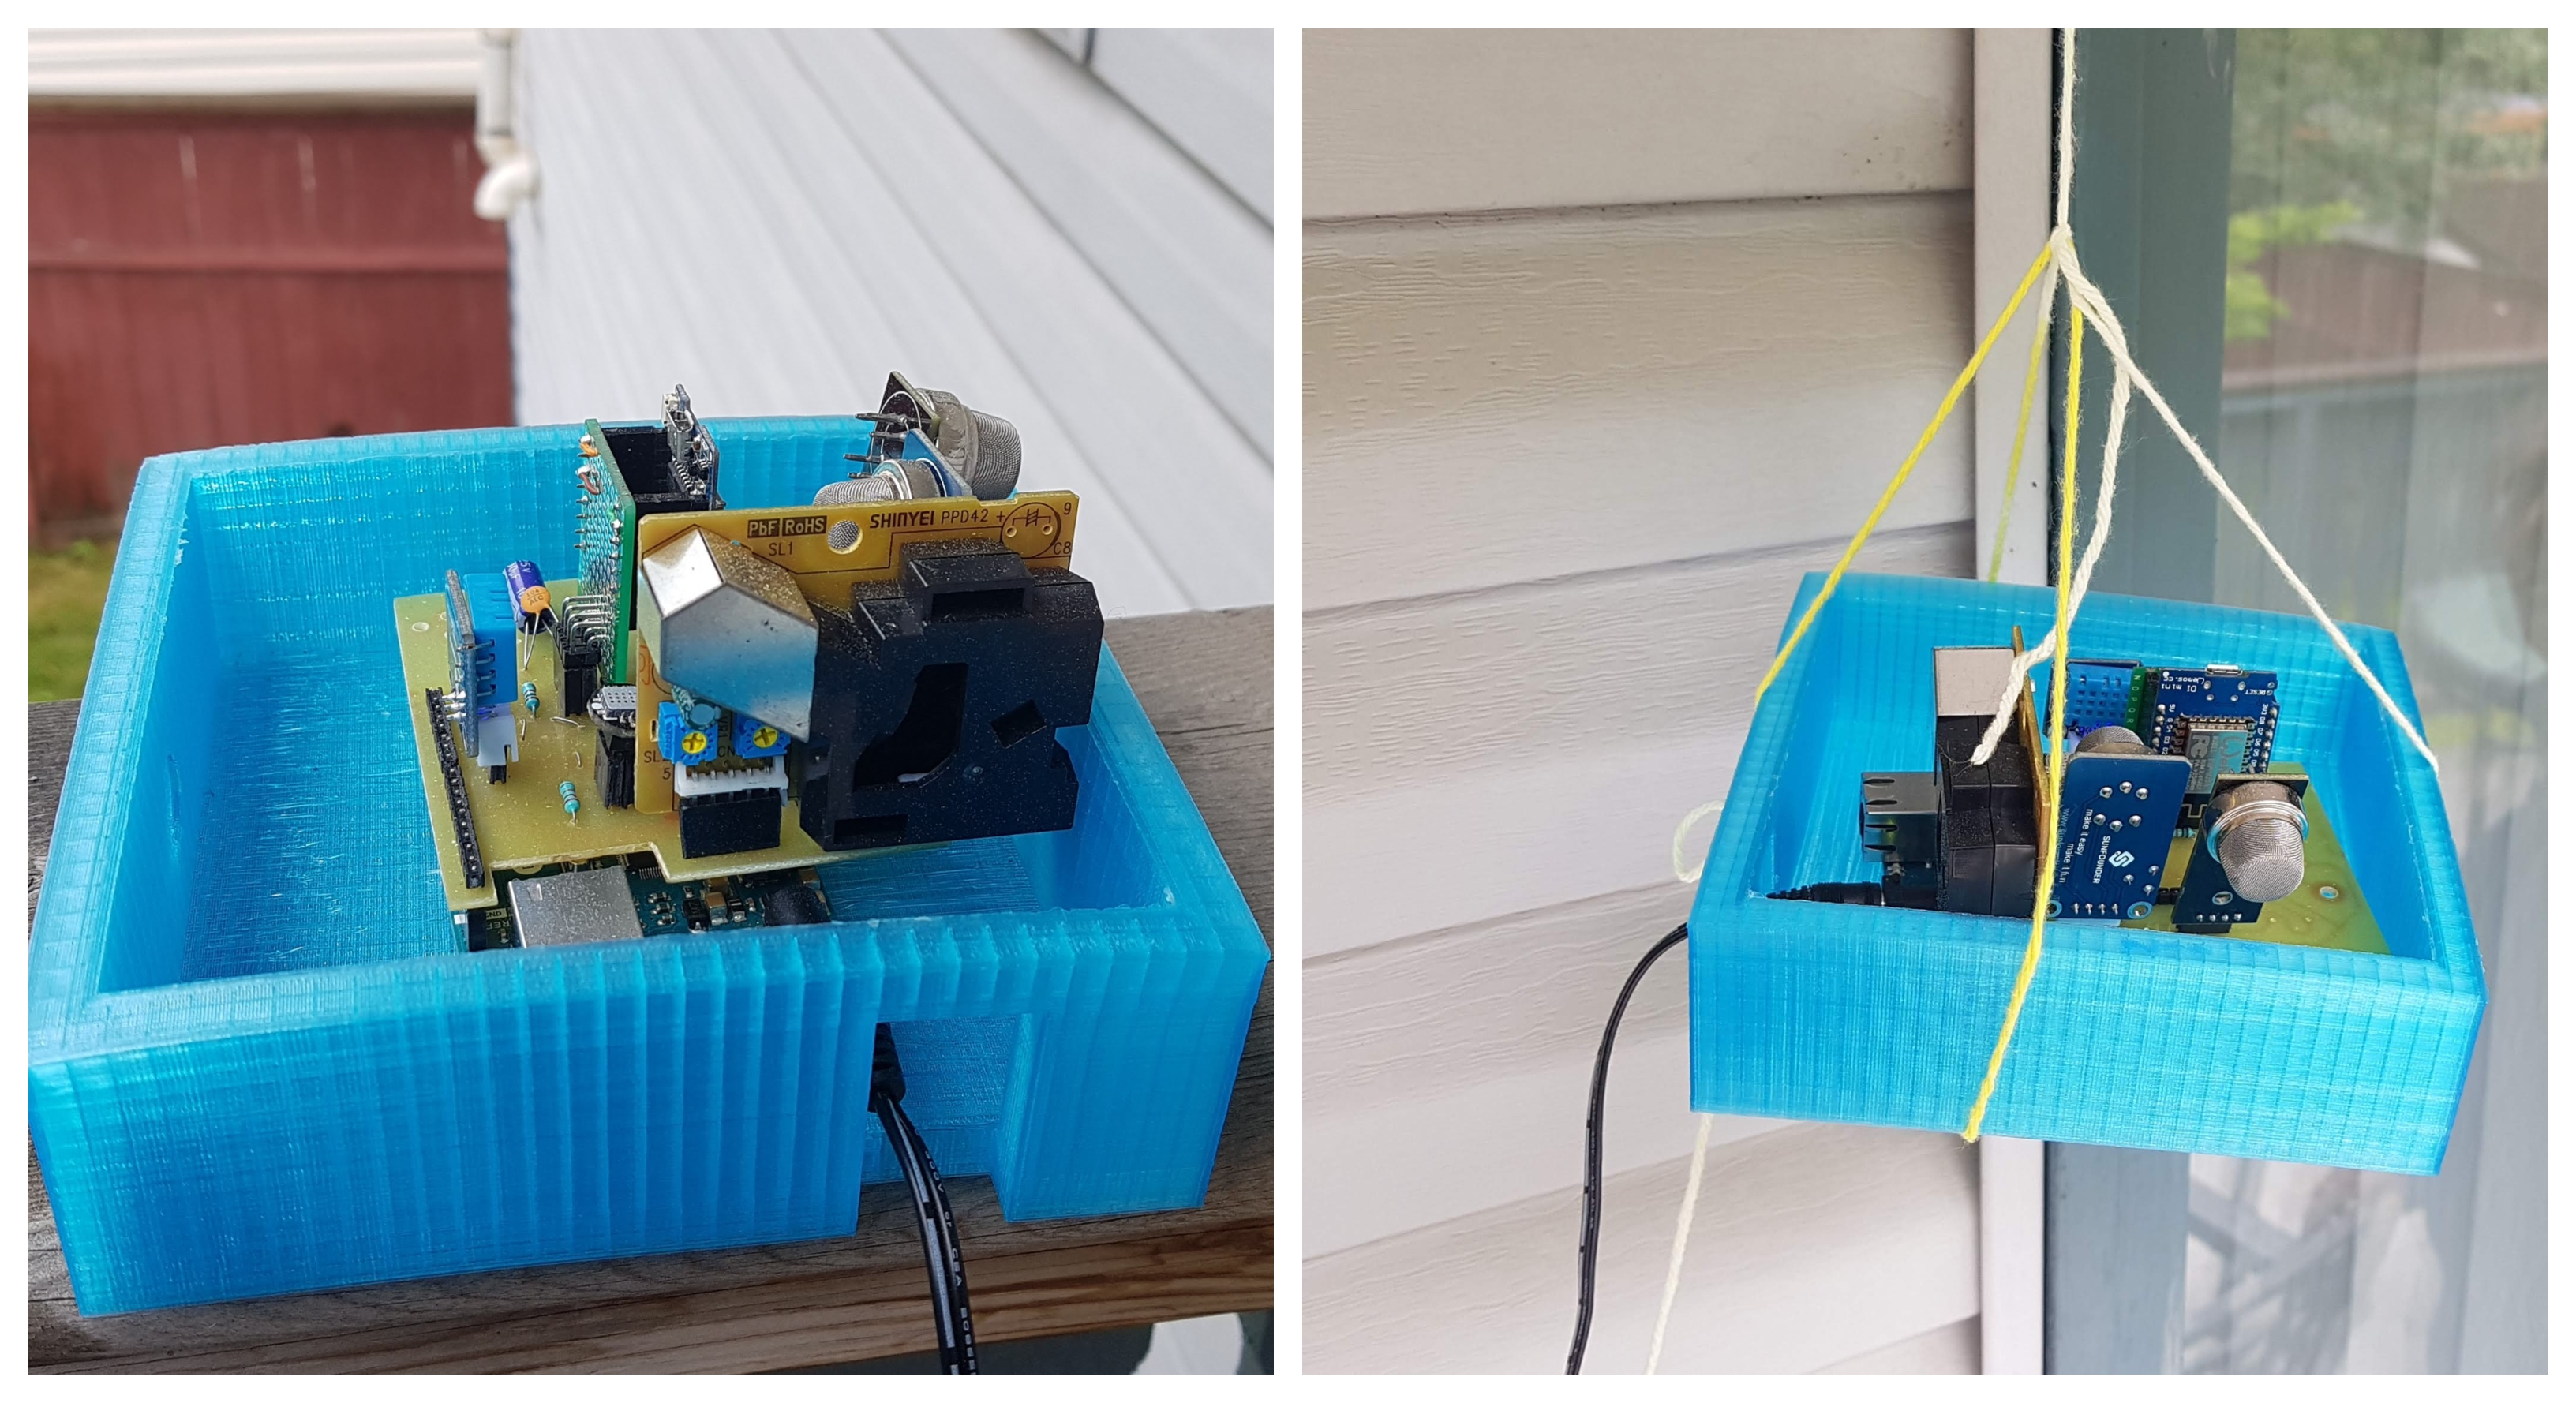
\includegraphics[scale=0.30]{images/figure20.jpg}
    \end{center}
    \caption{Deployed system at College Heights, Prince George}
    \label{deployed}

  \end{figure} 


  The main reason to conduct our deployment in this location was to have easy access and to check on the system regularly in case of any sensor faults or signal distortions. The measured raw values in the ThingSpeak database were compared to the reference values recorded at the downtown Plaza 400 building with the exception of carbon monoxide as it is not one of the pollutants measured at the Prince George reference station. Reference values for carbon monoxide were not available and hence were not analyzed. The Ozone, Particulate Matter (both $PM_{2.5}$ and $PM_{10}$), Nitrogen Dioxide, temperature and humidity data was collected and compared these to values at the Prince George reference station.


\section{Calibration}

The sensors that we are using to measure the pollutants are low-cost sensors and hence the accuracy of these sensors are expected to be less than those from the monitoring station operated by local or state agencies. To improve the reliability of the low-cost system we have used the MAT calibration procedure described in chapter 4. By applying the MAT procedure the final result is a calibration curve obtained by fitting the most appropriate equation to the set of data \cite{Stone2001}. Each sensor gives raw data values corresponding to the presence of gases or pollutant concentration.

The calibration procedure we used for the system is to collect the raw data values for two days and then apply the MAT calibration procedure. This will generate a calibration equation that is applied to the system to get the calibrated data. 
The calibration curve along with the reference data and sensor data is as shown in  Figure \ref{calozone} for Ozone, Nitrogen Dioxide and Particulate Matter. To explain the calibration procedure we use Ozone as an example. Figure \ref{calozone}  (top) shows three line graphs which include the reference data from the monitoring station, our sensor raw data, and the resultant calibrated curve. The calibration curve was obtained by applying linear regression. From the data graph, it can be seen that the Ozone raw data from our sensor system provided systematically lower values than the reference system and after applying the calibration equation the data could be aligned to be quite close to that of the reference system.



\begingroup
\setlength{\tabcolsep}{10pt} % Default value: 6pt
\renewcommand{\arraystretch}{2.0} % Default value: 1
\begin{table}[h]
  
  
  \begin{tabularx}{\columnwidth}{X|X}
      \hline
      Pollutant          & Regression equation \\
      \hline
  
   
    
    




    
    $O_{3}$   & $y = 1.42 * x + 0.04$  \\ 
    $NO_{2}$   & $y = 1.49 * x + 1.36$ \\ 
    $PM_{2.5}$   & $y = 1.31 * x + 0.27$\\ 
    $PM_{10}$   & $y = 1.59* x + 0.47$ \\ \hline
  
   
      
    
\end{tabularx}
 
  \caption{Regression equation for each sensor}
  \label{tableequation}
  \hspace{1 cm}
\end{table}
\endgroup











\begin{figure}[h]
  \begin{center}
    
  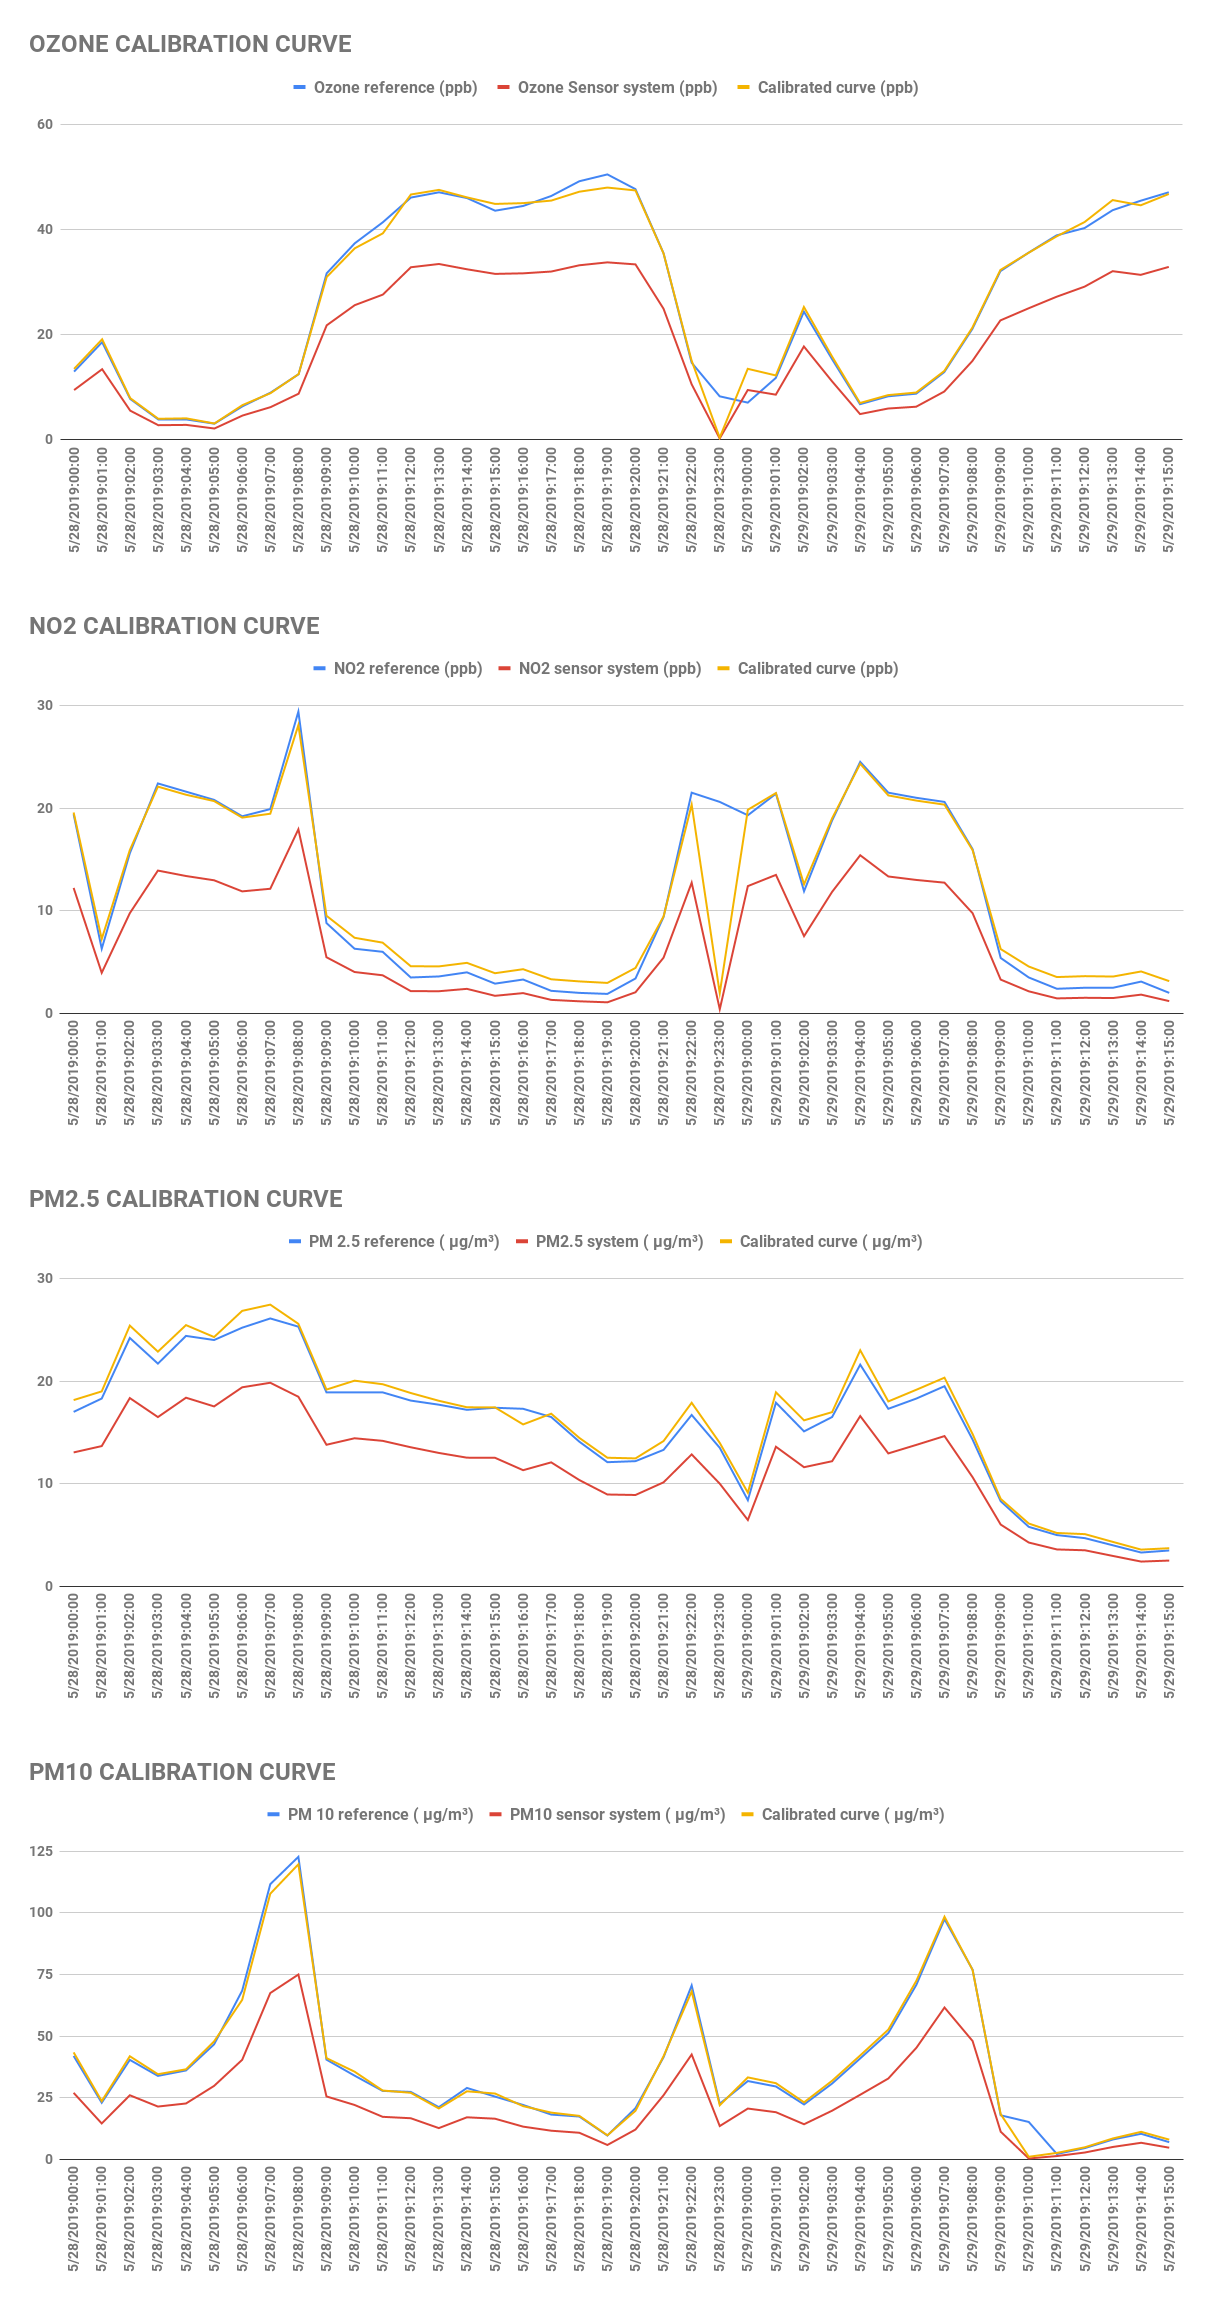
\includegraphics[width=118mm,scale=.50]{images/figure95.png}
  \end{center}
  \caption{Calibration curves for Ozone, Nitrogen Dioxide, and Particulate Matter.}
  \label{calozone}
  \hspace{1 cm}
\end{figure}

\clearpage
 %In the case of $PM$ sensor the output is a digital signal, called as Low Pulse Occupancy (LPO) which is converted to a concentration by applying an equation inside the Arduino. Later this concentration is applied to MAT for calibration.
 %For each case, we have shown the calibration curve as well as the regression fitting curve.





 We calibrated all the sensors (except for carbon monoxide and temperature and humidity) with the same linear regression procedure using MAT. 
 The calibration equation for our system is as shown in Table \ref{tableequation} where {\lq x\rq} refers to the raw value and {\lq y\rq }  refers to the calibrated raw value. The calibration equations in Table\ref{tableequation} were then supplied to the Arduino and then the system was used to measure the calibrated values.%In our case, Ozone shows a non-linear relationship above 200 ppb, in the future we could use polynomial regression or a better calibration method to make it more efficient. %To understand how good the regression line is to the data we have calculated the standard deviation of the residiuals or the root mean square deviation which is also given in the Table \ref{tableequation}. In the case of ${NO_2}$ there is a linear sensitivity curve so applying applying linear regression would give better results.  The $PM$ curve is linear till 50 ug/m3 and above that the response is attenuated \cite{wang2015laboratory}. %In the case of temperature and humidity sensor have not used the MAT tool since the DHT library did the calibration function.







   
   \section{Data Analysis}
  
  In this section, we will be comparing the collected data from our system to that from the reference system. We will be discussing the trends for each pollutant and will discuss possible reasons for the observed changes in concentration. The pollutants discussed are Ozone, Nitrogen Dioxide, $PM_{2.5}$ and $PM_{10}$ and later we will also be discussing the aggregated pollutant indexes (AQI and AQHI) which we discussed in Chapter 1.
  
  
  %We will be using multiple line graph plots to observe the data and will be investigating if there is any variations to these data.
  
  \subsection{Ozone}
As we have discussed in Chapter 1, Section 1.2,  the Ground-Level Ozone ($O_3$) is a secondary pollutant and is not normally directly emitted into the atmosphere. It is produced from a complex series of chemical reactions between other pollutants like Nitrogen Oxides (${NO_x}$) and volatile hydrocarbons (from combustion) in the presence of sunlight\cite{Environment2016}. The main sources of Nitrogen Oxides and volatile hydrocarbons that results in the production of Ozone in Prince George are industrial facilities, motor vehicle exhaust, and chemical solvents. The provincial objective for Ozone is less than or equal to 63 ppb to meet the air quality standards \cite{Environment2016}. 



Figures \ref{Ozone} and \ref{Ozone1} shows the Ozone readings obtained each day from May 30 to June 4, 2019. From Figures \ref{Ozone} and \ref{Ozone1} it can be seen that the calibrated sensor system shows a strong correlation with the reference system except for the last two days. The length of daylight on all the observed days was roughly around 16 hours and 30 minutes starting from 4.30 am in the morning to 9.30 pm in the evening \cite{daylight}. In all the measured days it can be seen that the concentration of Ozone is high during the daytime when compared to the late evening and night hours. The several reasons for having a high Ozone level can be due to:\cite{EnvironmentalQualitySectionMoE2012} 
\begin{enumerate}
  \item "An increase in Ozone precursors (other pollutants like Carbon Monoxide, Methane, Nitrogen Oxide in the presence of sunlight helps in the production of Ozone) in the upper atmosphere" 
  \item "More snow cover at higher elevation causing higher reflection of solar radiation back to the atmosphere" 
  \item "High level of ozone in the stratosphere being transported to the troposphere" 
  \item "A combination of all the three factors" 
\end{enumerate} 
 In our case,  the most likely factors are (1) and (3) or a combination of both. 
The possible reason for low concentration of Ozone during night hours is due to Ozone scavenging which occurs in the absence of sunlight \cite{EnvironmentalQualitySectionMoE2012}. Ozone scavenging is a chemical reaction between the ${NO}$ with ${O_3}$ that is present in the atmosphere to form ${NO_2}$ \cite{airqualityontario}. Even though the pollutants like ${NO_2}$ and volatile hydrocarbons in the presence of sunlight contribute to the production of ${O_3}$, ${NO}$ can destroy it \cite{airqualityontario} \cite{EnvironmentalQualitySectionMoE2012}.

 
Temperature is also considered to be a direct or indirect influence for an increase or decrease in the air pollution levels \cite{EnvironmentalQualitySectionMoE2012}. In the case of Ozone, higher temperature speeds up the reaction rate and increases the production of Ozone in the atmosphere \cite{coates2016influence}. For the measured days, the maximum temperature observed for the first three days (30th May to 1st June) is around 27 degrees Celsius and for the last three days (2nd June to 4th June) did not exceed 20 degrees Celsius. This might explain the observed higher concentrations of Ozone shown in Figure \ref{Ozone} when compared to the Figure in \ref{Ozone1}. The temperatures measured for each day by our calibrated system along with the comparison is included in the Appendix 



  \begin{figure}[h]
    \begin{center}
    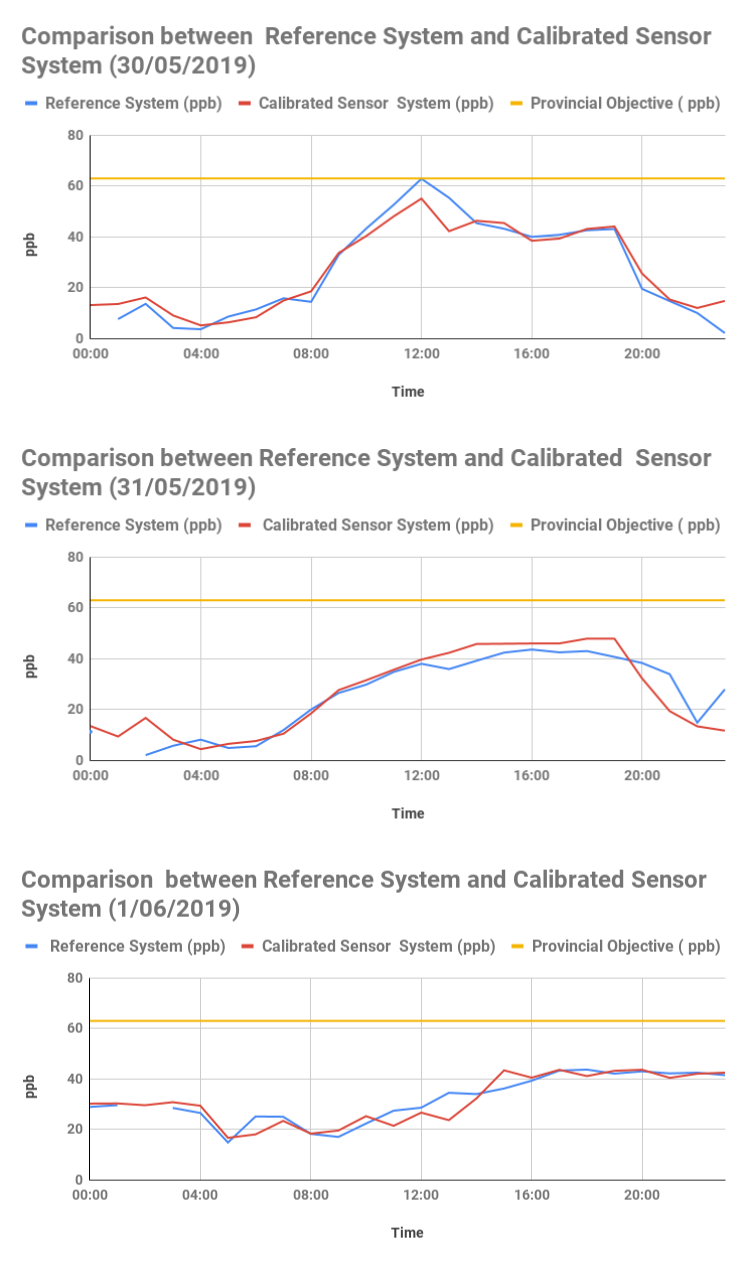
\includegraphics[scale=0.46]{images/figure104.png}
    \end{center}
    \caption{Comparison between Ozone values from sensor system and reference system from 30/05/2019 to 01/06/2019}
    \label{Ozone}
  
    %\hspace{1 cm}
  
  \end{figure}


 

  


  
  \begin{comment}
The maximum concentrations of Ozone are normally expected from May to August as these months have the longest hours of daylight which will increase the Ozone production \cite{Environment2010}. This means that the concentration of Ozone is high in days of 
  


  Our system measures this with the help of a semiconductor sensor MQ 131 which changes its conductivity with ozone \cite{technicalsheetozone}. The reference system in downtown uses an API model 400 ozone monitor for the city measurement\cite{Environment2010}. The Figure \ref{Ozonesensor} shows the picture of the Ozone sensor used for measurement at the reference station as well as in our low-cost sensor system.
  
  \begin{figure}[h]
    \begin{center}
    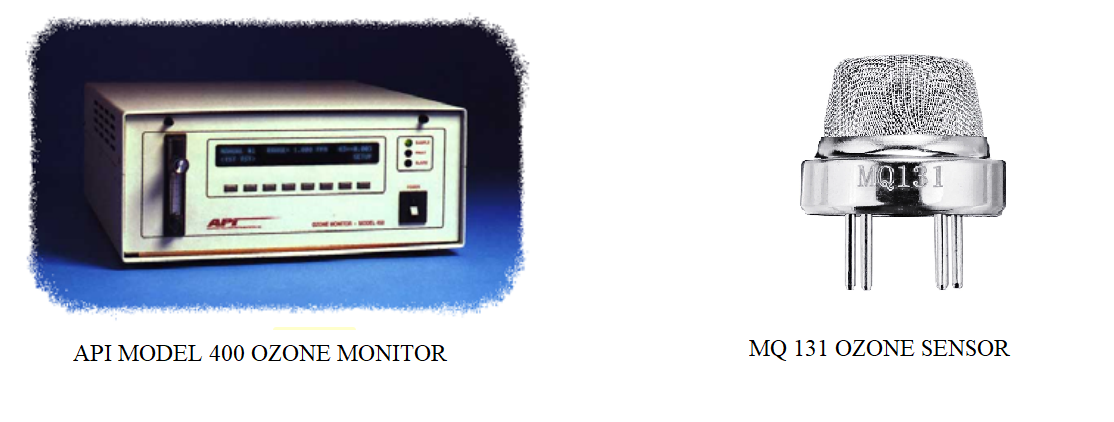
\includegraphics[scale=0.70]{images/figure30.png}
    \end{center}
    \caption{Ozone sensors used for measurement}
    \label{Ozonesensor}
  \end{figure}
  \hspace{1 cm}

\end{comment}



\begin{figure}[h]
  \begin{center}
  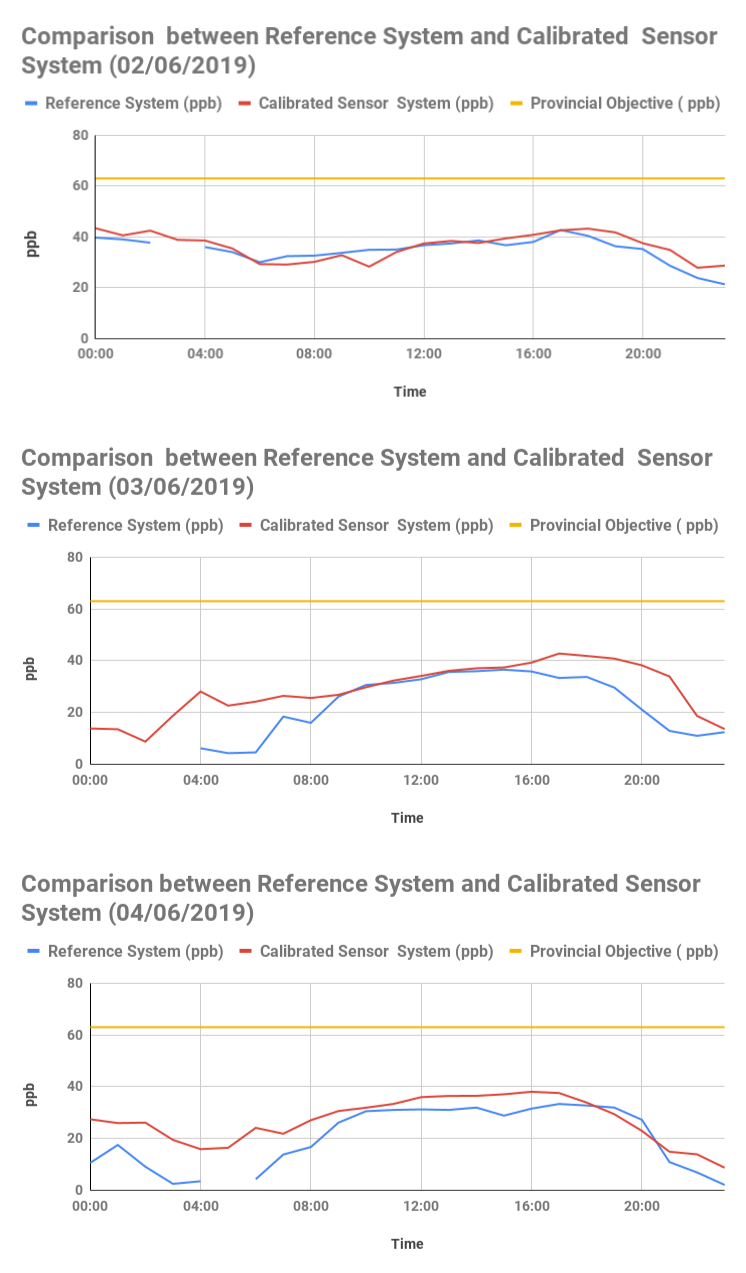
\includegraphics[scale=0.46]{images/figure105.png}
  \end{center}
  \caption{Comparison between Ozone values from sensor system and reference system from 02/06/2019 to 04/06/2019}
  \label{Ozone1}
  \hspace{1 cm}
\end{figure}
\clearpage

section for reference. It can also be seen that the first three days it was sunny when compared to the last three days where it varied from partly sunny to rainy. 

On all the measured days it can be seen that Ozone level have met the provincial objective standard which is less than or equal to 63 ppb \cite{Environment2016}. Over the observed period the calibrated sensor system was able to capture the changes in the concentration of Ozone  reliably. One outstanding issue is to determine when the system needs to do a recalibration procedure. As we have used a low-cost sensor system it is likely that there will be changes to the sensor performance over time. We have to characterize these sensor changes and the subsequent interval needs to be determined for recalibration procedures (eg: daily, weekly, quarterly). In general, we can say that the interval for recalibration for the sensor system needs to be looked in more detail. Nevertheless, it can also be seen that on the last two days the calibrated system showed differences in concentration when compared to the reference system. The environmental factors like temperature, relative humidity or concentration of confounding pollutants can result in change in sensor's sensitivity and reliability \cite{clements2017low}. This can be a possible reason for the sensor response differences seen for the last two days. 


% This could be a indication of a recalibration that is needed to be applied to the system. 



\begin{comment}

    The Nitrogen oxides (NOx) consist ofNitrogen Dioxide (NO2)and Nitric Oxide (NO).  This Nitric oxide reacts with ozone whichis present in the atmosphere to form Nitrogen Dioxide (NO2)is known as scavenging



  From the collected data it can be seen that the general trend for Ozone gas concentration rises during the daytime and is low during night as the presence of other pollutants are low in the night. It can be seen from the Figures \ref{Ozone} and \ref{Ozone1} that our sensor followed the trend similar to that of the reference system. For example, during the first day of our measurement, the Ozone concentration from our system ranges from 13.2 ppb in the early morning at 12:00 am then the concentration decreases to  6.32 ppb at 5:00 am. After this the concentration increases to 18.54 ppb at 8:00 am and later reaches its maximum of 55.09 ppb at noon. From noon till night the concentration decreases to 38.47 ppb in the evening to 11.98 during the night. A similar trend is followed for all the days of observations. The maximum concentration observed during the six days of measurements by our system was 55.09 ppb at 12:00 pm on the first day and the reference system also showed a maximum concentration of 62.90 ppb at the same time.

  
  The Figure \ref{Ozone} shows the line graphs of the first three days of the experiment and it can be seen that the concentrations are very close to the reference system. In Figure \ref{Ozone1} the graphs for the next three days found that on the last two days the values from the sensor shows more significant variation when compared to the first three days. This can be interpreted in two ways. The system might need to be recalibrated with a new regression equation so as to provide the output data close to the reference system. A second possibility is that, it could be a location-specific effect. Since the reference system is located downtown and there is a possibility of activities which can cause variations in change in concentrations. From this it can be concluded that a weekly calibration will be helpful to get concentration values similar to the reference station. Apart from that if the sensor system is kept in the area closer to the reference system the chances of getting values similar to reference system is more.
  
  %Considering the fact that we are using a low-cost sensor to measure the values from the surrounding and hence the need for calibration should be considered as a priority. 

\end{comment}

\subsection{Nitrogen Dioxide}



 \begin{comment}
  We have attempted to measure this pollutant with the help of low-cost sensor. 
 $NO_{2}$ was measured with the help of a popular silicon gas sensor called as MICS-2714 by calculating the sensing resistance. The reference system located in Prince George plaza 400 is API $NO_{x}$ monitor \cite{Environment2010} which uses chemiluminesence principle to measure the pollutant . The figure \ref{Nitrogensensor} shows the image of both the sensors for detecting the pollutant.
   
   
   \begin{figure}[h]
    \begin{center}
    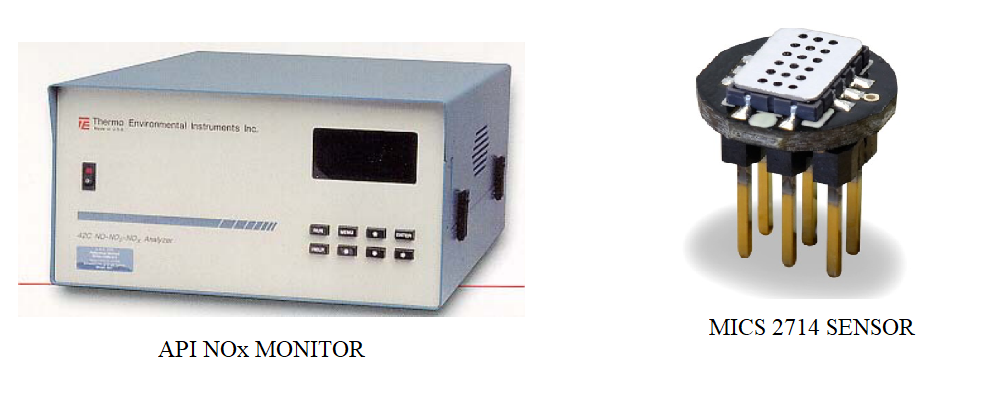
\includegraphics[scale=0.70]{images/figure31.png}
    \end{center}
    \caption{Nitrogen Sensor used for measurement}
  \label{Nitrogensensor}
\end{figure}
   
\end{comment}

%Nitrogen is the most abundant element in earth's atmosphere and is approximately 78\% by volume \cite{EnvironmentalQualitySectionMoE2012}. There are five forms of gaseous Nitrogen: Nitrogen (${N_2}$), Nitrogen Dioxide ($NO_2$), ammonia ($NH_3$), Nitrous Oxide ($N_2O$), and Nitric Oxide ($NO$). The combustion of motor vehicle exhaust, industrial process, fuel combustion for heating produces $NO$ which is easily oxidized to $NO_2$ or Nitrogen Dioxide \cite{EnvironmentalQualitySectionMoE2012}.

Nitrogen Dioxide is one of the main pollutants in urban areas that penetrates deep into the lungs and can cause pulmonary diseases. It is mainly produced from high-temperature combustion of fossil fuels, power plants and industrial activities \cite{EnvironmentalQualitySectionMoE2012}. The main sources of ${NO_2}$ in Prince George include combustion of fossil fuels in vehicles, power plants, other industrial processes \cite{Environment2016}. The provincial air quality objective for ${NO_2}$ is for concentrations to be  less than to 32 ppb \cite{Environment2016}. We have already discussed ${NO_2}$ in Chapter 1, section 1.2 about how high concentration of ${NO_2}$ can affect the human health. Using our system we have collected the data and have compared these to the data from the reference system. The collected sensor data in comparison with the reference system is shown in Figure \ref{Nitrogen} and \ref{Nitrogen1} that covers the data collection from May 30 through June 4, 2019. 

From Figures \ref{Nitrogen} and \ref{Nitrogen1}, the observed trend in the concentration of ${NO_2}$ is that it is higher in the morning and evening, and has lower levels in the afternoon. The higher levels in the ${NO_2}$ in the morning and late evenings could be the result of the oxidation reaction between $NO$ and $O_3$ in the absence of sunlight. One hypothesis for the observed changes in concentration of ${NO_2}$ could be related to variation in solar radiation, since in the absence of the sunlight there will be more oxidation reaction between $NO$ and $O_3$ \cite{Environment2010}. This process produces ${NO_2}$ as a night time reservoir and leads to increasing Ozone levels in the morning when photolysis resumes. This is the most likely reason for having a lower concentration of ${NO_2}$ during daytime \cite{rozbicka2014spatiotemporal}. Thus we could say that Ozone and ${NO_2}$ concentrations are often inversely related.  
    
On all the measured days there were long hours of sunlight and short nights with the first three days having a clear sky and last three days with partly sunny and light rain. It can be seen from the Figure \ref{Nitrogen} and \ref{Nitrogen1} that the concentration levels for ${NO_2}$ increases after 8:00 pm in the evening and decreases around 6:00 am in the morning and the reason for this could be related to the oxidation chemical reaction. The concentration of ${NO_2}$ for the last three days in Figure \ref{Nitrogen1} is lower than the first three days in Figure  \ref{Nitrogen}. This can be related to the temperature and humidity as the temperature on the last three days did not exceed more than 20 degree Celsius and there were rain showers on 3rd June which can be the reason for a very low concentration of ${NO_2}$ during the daytime. During the first three days the temperature was around 27 degree Celsius and at that time the concentration of ${NO_2}$ was around 25 ppb during its peak hours except for June 1st where the concentration of ${NO_2}$ was around 12 ppb during its peak hours. This shows a positive correlation between temperature and concentration of ${NO_2}$. The concentration of ${NO_2}$ did not exceed the provincial air quality objective of 32 ppb on any of the measured days but we do see that concentration  was ranging from 10-20 ppb on most days.

\begin{figure}[h]
  \begin{center}
  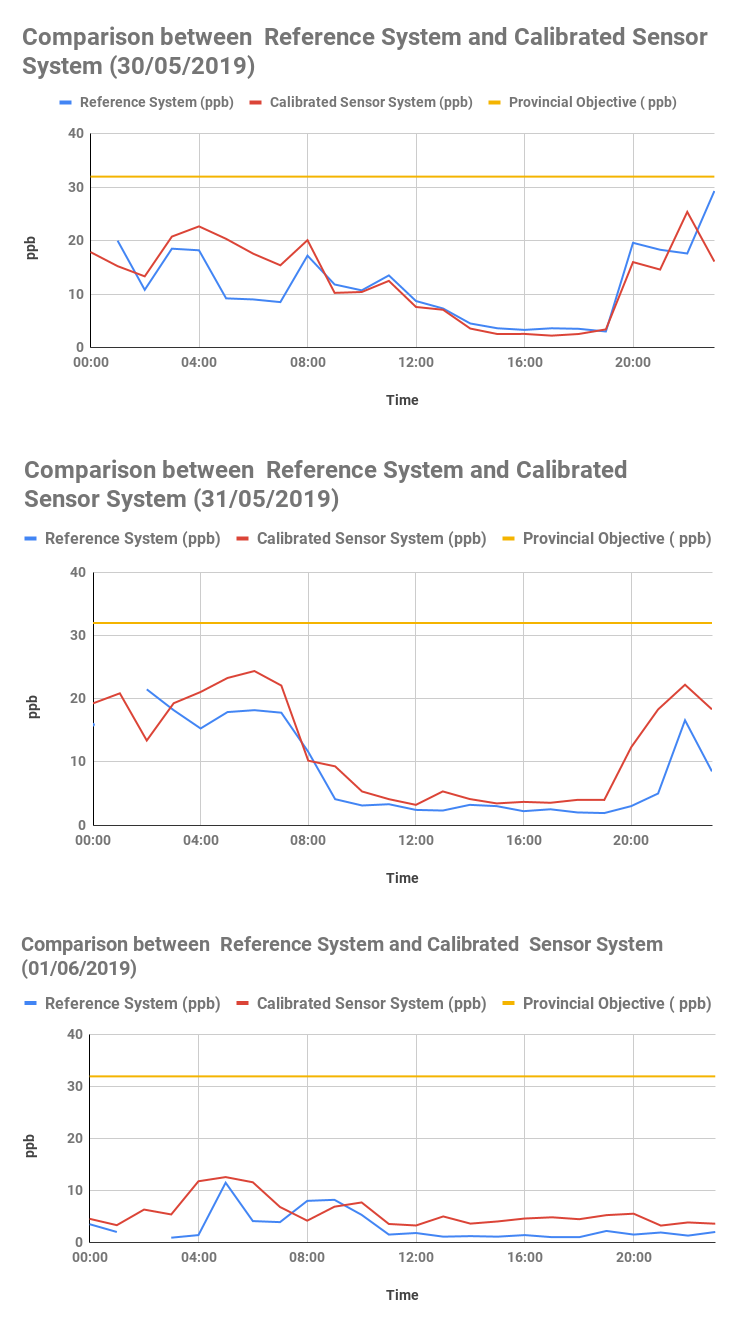
\includegraphics[scale=0.45]{images/figure106.png}
  \end{center}
  \caption{Comparison between Nitrogen Dioxide values from sensor system and reference system from 30/05/2019 to 01/06/2019}
\label{Nitrogen}

\end{figure}
\clearpage

\begin{figure}[h]
  \begin{center}
  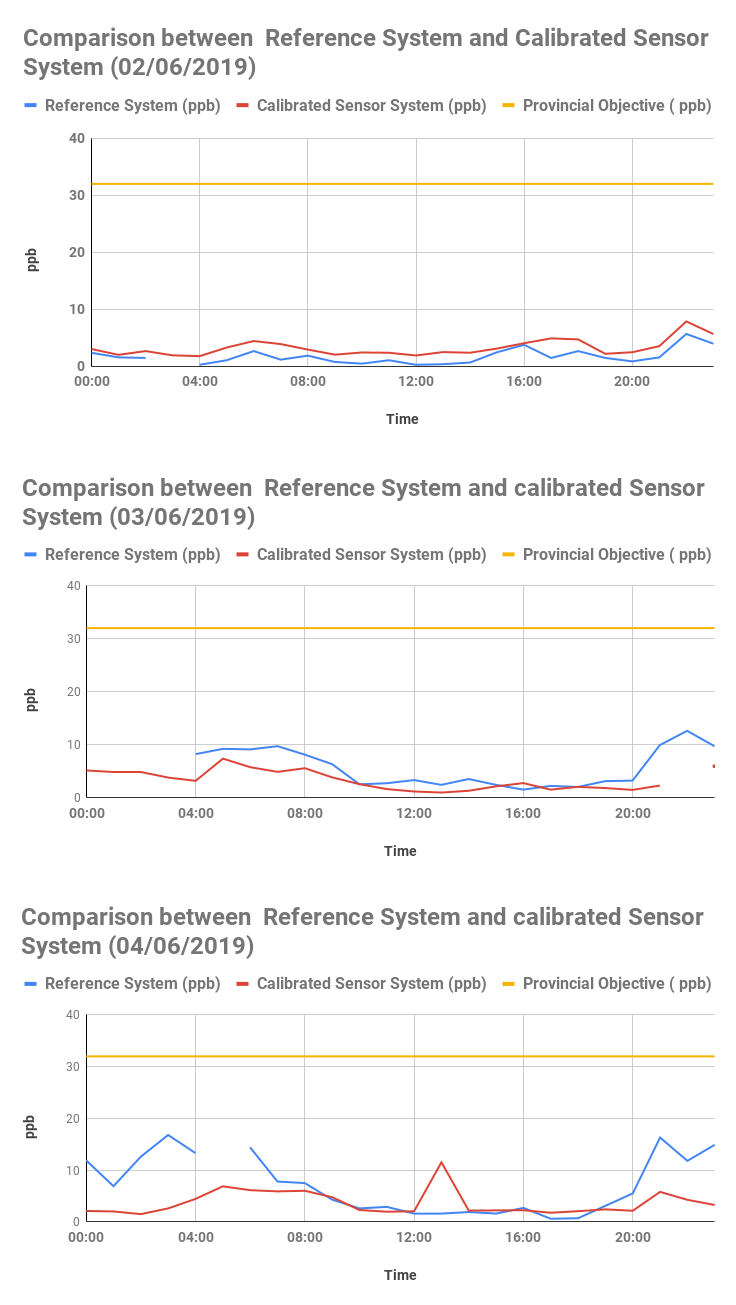
\includegraphics[scale=0.45]{images/figure107.png}
  \end{center}
  \caption{Comparison between Nitrogen Dioxide values from sensor system and reference system from 02/06/2019 to 04/06/2019}
  \label{Nitrogen1}

\end{figure}
\clearpage






% In the city of Prince George, the highest level of ${NO_2}$ is seen during winter months (January and February) and lowest in July \cite{Environment2010}. This increase in the concentration of ${NO_2}$ during winter is because of increased use of heating sources or heating fuels and another reason is due to less solar radiation which will reduce the breakdown of ${NO_2}$ to Nitric oxide ${NO}$ which in turn increases the build-up of ${NO_2}$ in the atmosphere \cite{Environment2010}.The maximum value measured from our sensor system was 25.39 ppb on the first day. The values measured from last two days comes under 12 ppb. The values are seen to be fluctuating through out the graphs. It can be interpreted from the graph that even though the values of the pollutant at each point of time is different from the reference system but for the first three days the trend is followed. At the same time it can also be seen in the figure \ref{Nitrogen1} that the values from both the system have less similarity.

    
    %On the first day our system measures a value of 22.67 ppb at 4:00 am and then the value decreases to around 10.23 ppb by 9:00 am and further decreases to 3.55 ppb at 2:00 pm. The measured value rises to around 16 ppb by 8:00 pm and by 11:00 pm the value is 25.39 ppb.

    %The general trend for the value of ${NO_2}$ is high during the night and low in the day time. This trend is followed by the reference system as well and is clearly shown in the Figure \ref{Nitrogen} and \ref{Nitrogen1}. 

    %This gas is generated from the liberation of Nitrogen present in the fuels and is considered as a serious pollutant to the environment \cite{Salonen2019} \cite{govcanada}.
 

    
    
    
    
    %This change in concentration of Nitrogen dioxide can understood by the variation in solar radiation during a typical day \cite{Environment2010}. A lesser amount of radiation from sun slows down the breakdown of ${NO_2}$ to ${NO}$ which accumulates ${NO_2}$ in the stratosphere \cite{EnvironmentalQualitySectionMoE2012} \cite{Environment2010}. This can be seen in the graphs in both the reference value as well as in our sensor value. Another possible reason for high values can be related to heavy traffic as the graph shows the concentration hits it's peak concentration around 8.00 am which is considered to be office time for most people in the city. 
 


    The results from our observations show that our ${NO_2}$ sensor had a strong correlation with the reference station for the first two days and later there was a fluctuation in the measurements. In absolute terms the differences are similar in all of the days and later days had less variability. There can be several possible reason for the variation in values. This can be either related to the drifting of sensor performance or the impact of environmental factors on the sensor. Another factor for less correlation can be the cross-sensitivity effect as all the sensors are placed together there will be the effect of other pollutant values which will cause a change in measurements \cite{clements2017low}.

 Next factor could be change in temperature and relative humidity as these will reduce the sensitivity especially at higher humidity conditions leading to decrease in sensitivity\cite{clements2017low}. Finally the location of the sensor system can also contribute to this as the system was placed in University Heights and the reference system is in Downtown.
    



 \subsection{Particulate Matter}


Particulate Matter includes those particles whose size range from 0.001~{\textmu}m to 100~{\textmu}m. In Prince George, pulp mills and saw mills are primary sources for their emission, and during the winter,  road dust also adds to this primary pollutant category as winter street sanding is done around that time \cite{Champagne1996}. The activities like street sweeping also contributes to the particulate matter pollution. Studies show that PM levels are usually low during the winter season and are higher during late winter and summer season \cite{EnvironmentalQualitySectionMoE2012}. In Prince George particulate matter pollution is a matter of serious concern and a variety of studies are being conducted. The provincial objective for $PM_{2.5}$ are 25~{\textmu}g$/m^3$ and for $PM_{10}$ are 50~{\textmu}g$/m^3$ for the maximum daily (24-hours) mean for the year \cite{Environment2016}. We will discuss the observed trends of the collected sensor data and the reference data from 30th May, 2019 to 4th June, 2019.

Both $PM_{2.5}$ and $PM_{10}$ are location-dependent pollutants and can drastically change in concentration due to local activity. Data from the sensor system and the reference data from downtown for both $PM_{2.5}$ and $PM_{10}$ are shown in \Crefrange{PM10}{PM2.5.1}. Figures \ref{PM10} and \ref{PM10.1}, presents $PM_{10}$ data, and it can be seen that the values in the early morning and in the evening are the highest each day except for last two days in Figure \ref{PM10.1}. The daytime (11:00 am to 7:00 pm) concentration of $PM_{10}$ is observed to be low generally. This is true in the case of the reference station values as well. On one of the measured days (on 03/06/2019), there was precipitation in the early morning from 12:00 am to 7:30 am and that might be the reason for lower concentrations of $PM_{10}$ for that day and next (04/06/2019). The first two days showed a higher $PM_{10}$ concentration compared to the rest of the measured days and can be be seen from the Figure \ref{PM10} and \ref{PM10.1}. This higher concentration in $PM_{10}$ can be associated to wind condition around that time. The first two days had calm winds around 4 km/h that makes it difficult to flush the $PM_{10}$ pollutant out of the airshed and results in higher concentrations \cite{EnvironmentalQualitySectionMoE2012}. The rest of the days the wind speed varied from 10 to 20 km/hr and can be a reason for lower concentrations of $PM_{10}$ when compared to the first two days. The provincial objective of $PM_{10}$ (50~{\textmu}g$/m^3$) was exceeded on the first three days.


In the case of $PM_{2.5}$,  from the data in Figures \ref{PM2.5} and \ref{PM2.5.1} we can see similar trends from the sensor system data as the reference system except for some variations which happened for a short interval of time and these might be associated with local activities near the reference system or the sensor system. The first two days in Figure \ref{PM2.5} showed a higher value for both sensor system and reference compared to the rest of the measured days. This can again be related to calm wind condition on for those two days when compared to the rest of the days. 


In the \Crefrange{PM10}{PM2.5.1}, it can be seen that for most of the days our sensor system measured higher values for both $PM-{2.5}$ and $PM_{10}$. This could be because the reference system is placed in a high roof top elevation and our sensor system is at a low roof top elevation. This could be one of the reason why our system shows higher value than the reference system. During the year 1996 a short-term experiment was conducted by Ministry of Environment to understand if there is any difference in the street-level pollution and was compared to the Plaza site (elevated building). The values collected from street levels shows that the particulate matter values were 30$\%$ higher than the Plaza value \cite{Environment2010}.


\begin{figure}[h]
  
  \begin{center}
  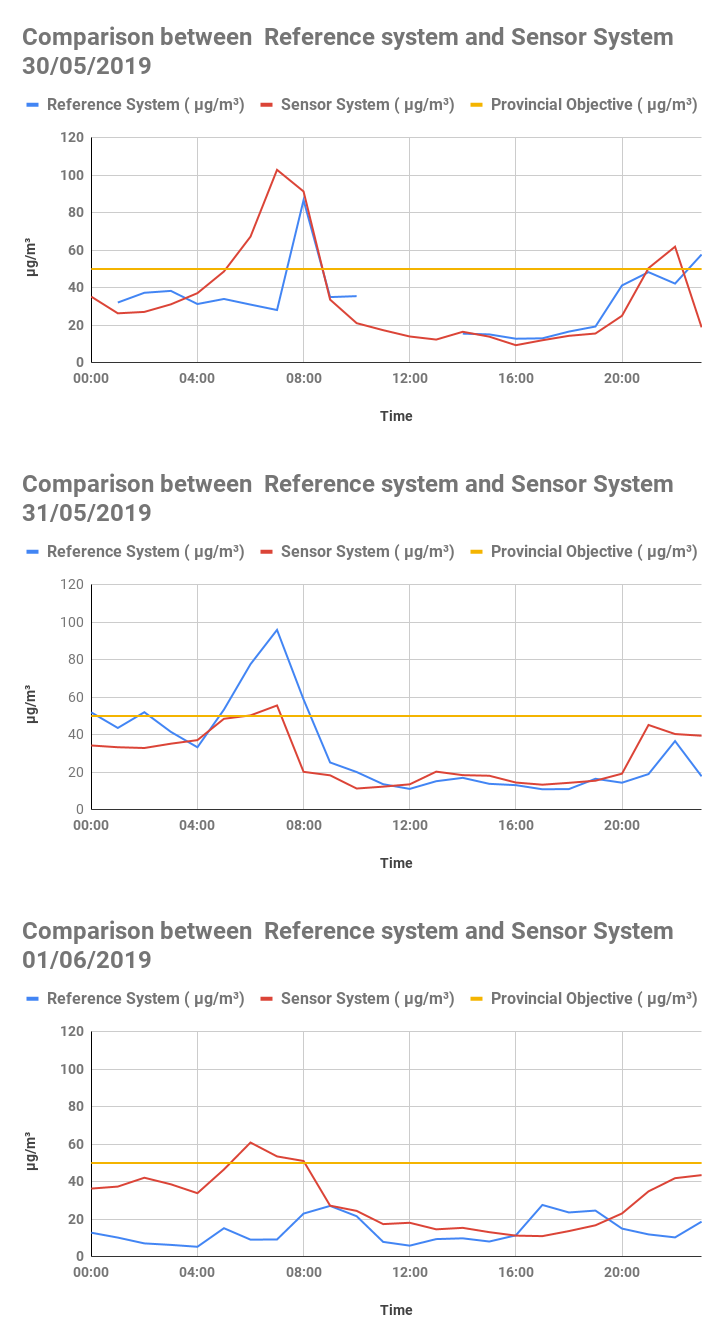
\includegraphics[scale=0.42]{images/figure99.png}
  \end{center}
  \caption{Comparison between $PM_{10}$ values from sensor system and reference system from 30/05/2019 to 01/06/2019}
\label{PM10}
\hspace{1 cm}

\end{figure}
\clearpage


\begin{figure}[h]
  \begin{center}
  \includegraphics[scale=0.43]{images/figure98.png}
  \end{center}
  \caption{Comparison between $PM_{10}$ values from sensor system and reference system from 02/05/2019 to 04/06/2019}
\label{PM10.1}
\hspace{1 cm}
\end{figure}
\clearpage







\begin{figure}[h]
  \begin{center}
  \includegraphics[scale=0.43]{images/figure100.png}
  \end{center}
  \caption{Comparison between $PM_{2.5}$ values from sensor system and reference system from 30/05/2019 to 01/06/2019}
\label{PM2.5}
\hspace{1 cm}
\end{figure}
\clearpage


\begin{figure}[h]
  \begin{center}
  \includegraphics[scale=0.43]{images/figure101.png}
  \end{center}
  \caption{Comparison between $PM_{2.5}$ values from sensor system and reference system from 02/05/2019 to 04/06/2019}
\label{PM2.5.1}
\hspace{1 cm}
\end{figure}

\clearpage





%The factors which contributed to $PM_{10}$ are similar to that for $PM_{2.5}$ like combustion, road dust, industries etc. The particle size of $PM_{2.5}$ are more finer than $PM_{10}$ and has more health effects. On inhaling these particles can causes cardivascular diseases and other breathing problem. From the Figure \ref{PM2.5} it can be seen very clearly that on all the measured day the values are low and have not exceeded 40 $ug/m^3$. The reason for such low values can be also related to meterological factor, wind direction or the location where it is measured. The graphs for $PM_{2.5}$ shows a good similarity to the reference system values.


From this, we can say that as our sensor station is at a low roof top elevation could be a reason for showing higher concentration. Another possible factor for the difference in values in reference and sensor system can be the location where our sensor is placed and the wind direction. As our sensor was in a residential area on a roof top of a house (in College Heights, Prince George) the activities happening in the residential area could affect the concentration of Particulate Matter. The activities taking place in the downtown area are different to that of the residential area and the system could measure different values.


Both $PM_{10}$ and $PM_{2.5}$ showed higher values for the first two days when compared to the rest of the days. Windspeed and precipitation are two factors that affect both $PM_{10}$ and $PM_{2.5}$. High windspeed will contribute to dispersion of the particles into the atmosphere. The higher windspeed will help to transport the particles to a further region. Precipitation can also have a similar effect on Particulate Matter. Precipitation helps to settle down the dust particles and will result in lower concentrations.



In the Figure \ref{PM10.1} and \ref{PM2.5.1} we could see several peaks for both of the Particulate Matter pollutants that our sensor system measured. This is very tricky to identify, as unlike other pollutants present in the atmosphere both $PM_{10}$  and $PM_{2.5}$ pollutant level are very dependent on location and any local activities has significant effect on the values.









\subsection{Air Quality Indexes}


As discussed in Chapter 1, section 1.2, the air quality indexes are the numbers that aid the general public in understanding the air quality in the area they live in. AQHI is a cumulative tool that helps to recognize the cumulative nature of poor air quality on health \cite{hasselback2010air}.  AQI is a single number that is calculated by selecting the maximum sub-indices of individual pollutants. In our analysis, we have calculated the AQI (Air Quality Index) and AQHI (Air Quality Health Index) indexes from the collected values of both our system and the reference system by using the equations 1.1, 1.2, and 1.3 from Chapter 1, section 1.2.

In Canada, the most commonly used index for the public is AQHI, which is a number scale which defines how the air quality affects the human health \cite{AQHICAN}. The value of AQHI ranges from 1 to 10+ (highest). The pollutants included in the calculation of this health index are $NO_{2}$, $PM_{2.5}$ and $O_{3}$. We have calculated the AQHI for each hour and then we took the average for the day, and have compared this with the AQHI provided by the Environment Canada based on the data from the reference system at Plaza 400. Figure \ref{AQHIAV} shows the comparison between these values. It can be seen from the Figure \ref{AQHIAV} that AQHI value is a combination of all the three pollutants. Ozone contributed the most to AQHI value in all the measured days for both sensor and reference system.

\begin{figure}[h]
  \begin{center}
  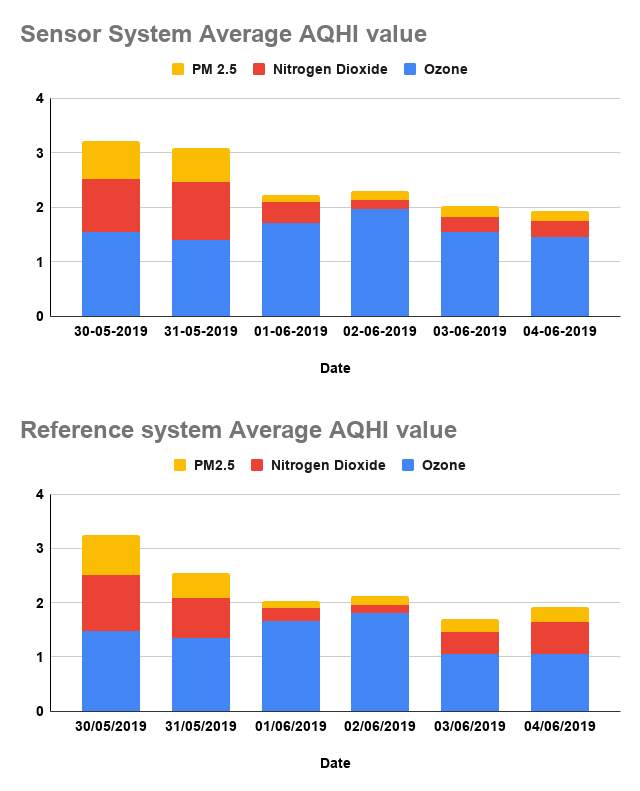
\includegraphics[scale=0.52]{images/figure108.png}
  \end{center}
  \caption{Comparison between average AQHI from both reference and sensor system}
  \label{AQHIAV}
  \hspace{1 cm}
\end{figure}


The overall AQHI for the observed days falls under the first category, which is the low-health risk which is discussed in Chapter 1, Section 1.2. From Figure \ref{AQHIAV} it can be seen that the AQHI values for all the days shows a good correlation to the reference system. On all the measured days the risk factor associated with health is low as per the index chart provided by the government \cite{AQHICAN} which is discussed in Chapter 1, Section 1.2.

 The next index that we calculated is the AQI in which we have used the measured pollutants from the sensor system and the reference system. The pollutants used of measurement for the AQI are $NO2$, $PM2.5$ and $O3$ and we have not used $CO$ as the reference system in Prince George did not provide the value. AQI communicates the air quality of an area based on the single worst pollutant. The Figure \ref{AQIAV} shows the graph of the daily averaged AQI values.

 \begin{figure}[h!]
  \begin{center}
  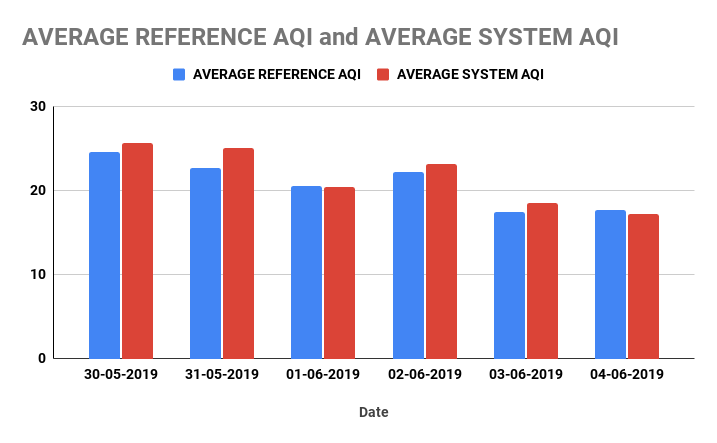
\includegraphics[scale=0.53]{images/figure92.png}
  \end{center}
  \caption{Comparison between average AQI from both reference and sensor system}
  \label{AQIAV}
  \hspace{1 cm}
\end{figure}

It can be seen in Figure \ref{AQIAV} that on majority of the days our sensor system shows a slightly higher AQI value as compared to the reference system. These AQI values fall into the first category of the scale provided by the government which means the air quality during the measured days was 'Good'. The pollutant which contributed the most to AQI is Ozone.
BY looking at the correlation in reading of the AQHI and AQI index measurements in Figure \ref{AQHIAV} and \ref{AQIAV} shows how well the system could capture the values after calibration. 


In this work, we have built a sensor system which measures the pollutants specific to Prince George. The system which we have built is very simple, easily replicable and the sensors used are low-cost and readily available.We have also implemented calibration with the help of MAT tool and after that put our system out for six days and collected data. The measurement of each pollutant showed a good correlation to the reference system except for $PM_{2.5}$ and $PM_{10}$. The comparison of AQI and AQHI shows that our system was able to reproduce values similar to the reference system. One main concern of the system is the calibration procedures and the interval for recalibration. In order to understand this we need to collect more data. Overall we could say the system showed a good correlation to reference system  and the calibration procedure could be improved. We will be discussing more about possible future work in the next chapter.
